%!TEX root = ../thesis.tex
%Adding the above line, with the name of your base .tex file (in this case "thesis.tex") will allow you to compile the whole thesis even when working inside one of the chapter tex files

\singlespacing
\chapter{Conclusions and Future Work} 

\label{chap:6}

\doublespacing
The first goal of the this thesis was to derive CME masses from observation that have the smallest and most reliable uncertainty to date, and to use this information to calculate a better estimate of CME energies and the first observational quantification of the Lorentz force acting on a CME.
The second goal of this thesis was to increase the understanding of the relationship between CMEs, CBFs and radio bursts. This was achieved through evidence for a shock driven by a CME flank, resulting in the CBF and type II, type III, and herringbone radio bursts. n this chapter, I will summarise and conclude this research and outline the future of this study
\clearpage

\section{CME Masses and Energies}

\subsection{Principle results}

The goal of the this thesis was firstly to derive CME masses from observation that have the smallest and most reliable uncertainty to date. This was achieved using the two vantage points of the STEREO Ahead and Behind spacecarft, allowing CME geometry, and the associated mass underestimations, to be fully characterized. This then allowed a better estimate of CME energies and the first observational quantification of the Lorentz force acting on a CME. The principle results are as follows:
\begin{itemize}
\item The first assumption of nearly all CME investigations is that the CME is confined to the 2D sky-plane. These leads to two sources of mass underestimation which primarily arise from the geometrical sensitivity of the Thomson scattering equations for the solar atmosphere. Firstly, if the CME propagates propagates at some angle away from the sky-plane, but we do not take into this angle into account, then we will underestimate the mass. Knowledge of the propagation angle from STEREO A and B observations allows us to eradicate this uncertainty. Secondly, all CME material is confined to a 2D plane at some angle $\theta$. This underestimation cannot be eradicated but we can characterise its effects by simulating a CME with angular width $\psi$ and homogenous density distribution. This allows an estimate of the simulated observed mass and a comparison of this to the actual mass. For any CME width $\psi$ at a sky-plane angle $\theta$ we may calculate the CME mass underestimation when we deproject the CME mass onto its plane $\theta$. A surprising result from this is that for all angular widths $\psi$, deprojection estimates exactly the CME mass when propagation is at an angle $\theta=60^{\circ}$.

\item In the past CME mass uncertainties from the geometrical unknowns described above were either extremely large at more than 50\% \citep{vou00} or entirely unquantifiable. Adding to this all the other sources of uncertainty (coronal composition and interactions with streamers) results in CME mass estimates that are entirely unusable in a scientific analysis. With the capabilities of the STEREO spacecraft, the geometrical mass uncertainties of the CME occurring on 12 December 2008 were reduced to 10\%, a dramatic improvement over previous results. The biggest source of uncertainty was the interaction of this CME with a streamer, adding a further 15\%. Taking everything else into account the final mass uncertainty came to 30\%, which is both smaller and more reliable than any uncertainty given previously. The final total mass of the CME came to
$3.4\pm1.0\times10^{15}$\,g, perhaps the only quotation of mass with an uncertainty in the literature. In an ideal case of a CME that has no background streamer interactions the uncertainty could be reduced even further.

\item This research included the first quantification of the Lorentz force acting on the CME during its early phase propagation. At $3.4\pm2.2\times10^{14}$\,N, it was shown that this is the most dominant force on a CME at $3\,R_{\odot}$, being greater than gravity and drag due to the solar wind. This is the first direct evidence for Lorentz force dominated dynamics, which has been only indirectly shown in previous studies \citep{bein2011}. The quantification of this force is also important for constraining parameters of MHD models of CMEs. There are a variety of models of CMEs which successfully describe formation of a flux rope and its eruption into interplanetary space. These models employ a number of forces, given by the MHD momentum conservation equation, to propel the CME out of the low corona. The most important of these forces for doing work against the Sun's gravitational potential is the Lorentz ($\mathbf{j}\times\mathbf{B}$) force. While all models include a Lorentz force treated explicitly through currents and magnetic fields, or implicitly only through magnetic field, the sizes of the force in the models is entirely unconstrained. MHD models of CMEs have the freedom to choose any size Lorentz force because no work had been done on the actual size of this force. For example, \citep{chen1996} predicts a Lorentz force of X\,N during early phase propagation. This would seem to orders of magnitude too high, and further observational investigations of the forces on CME may show this.

\end{itemize}

\subsection{Future Work}

\subsubsection{CME Mass and Energy Catalogue}

There are a variety of catalogues that list CME times and kinematics for all events detected by LASCO up to the present time (REFERENCES). None of these catalogues include any measure of CME masses. This is possibly due to the difficulty in unambiguously identifying the CME in coronagraph images. A current investigation is underway to test the feasibility of automatically calculating all the masses of all CMEs in the LASCO catalogue. Such an endeavor would require accurate detection of all CME material in the images. The automatic detection routines under development by Byrne are a possible candidate to employ automatic mass calculation routines. The Byrne algorithm has the possibility of providing masks for the total CME area such that a summation of its mass content may be achieved. These masks are shown in Figure~\ref{fig:masks}. These masks use multi-scale filtering to detect the area of the CME in the image. A conversion of the image to pixel values of grams, as described in Chapter 4, and summation of the all pixels would yield the total CME mass.

\begin{figure}[h!]
\begin{center}
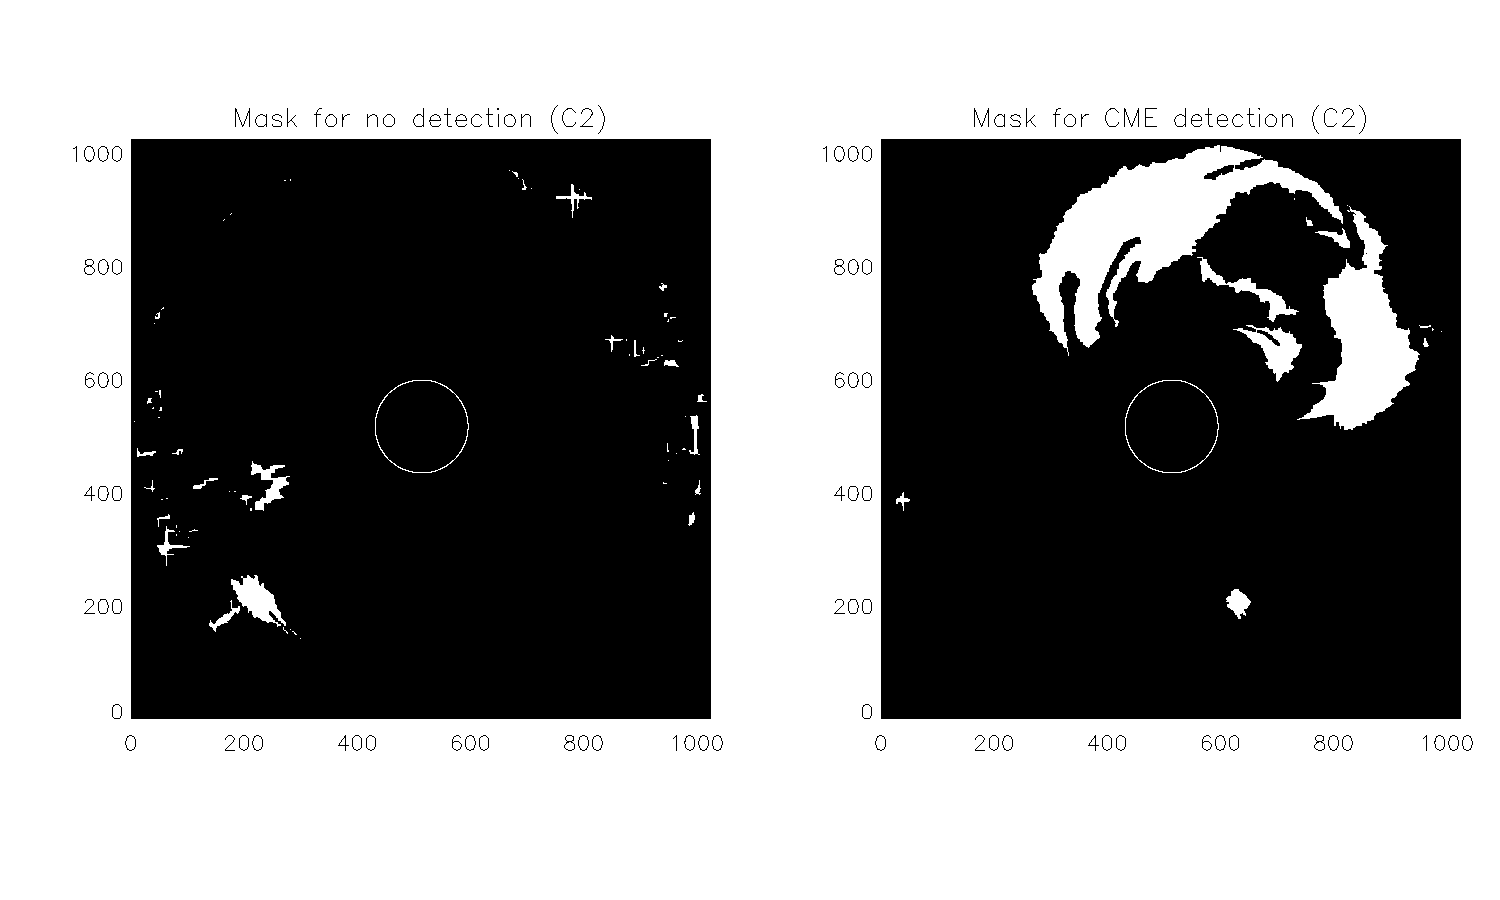
\includegraphics[scale=0.6, trim=2cm 2cm 1cm 1cm]{masks.pdf}
\caption{Sample C2 masks for no-detection (left) and CME-detection (right). The no-detection masks has some spurious blobs, possibly due to cosmic rays and small ejections of plasma. The CME detection covers most of the CME body, but masks the center due to presence of CME core? Circle shows solar limb.}
\label{fig:masks}
\end{center}
\end{figure}
%----------------------------------------------------%
%			  Describe method
%
The method was tested on a particularly active period of CME eruptions from 25 April 2010 to 2 May 2010, observed by LASCO C2 and C3. The detection mask was applied to each image in the sequence between the dates. In the majority of images there are no detections (Figure~\ref{fig:masks}(left)) and if a CME is in the image it will be exposed in a mask similar to Figure~\ref{fig:masks}(right). Each image is base differenced and converted to pixel values of grams using the sky-plane assumption. The pixels are summed such that one image represents one mass value for each image in the sequence i.e., the image sequence allows us to calculate a mass time-series, shown in Figure~\ref{fig:mass_v_time}. The top panel shows a mass time series on a linear scale, the CME detections of a standard $\sim$$10^{15}$\,g can be seen in the time series of both C2 and C3. The method is quite successful in calculating a reasonable mass value for moderate to large CMEs ($\sim$$10^{15}-10^{16}$\,g). 
%----------------------------------------------------%
%			       Initial trial
%
A more appropriate representation is given in Figure~\ref{fig:mass_v_time}\,(lower), where the y-axis is logged. Realistically, all of the mass plots should be logged given that CME masses tend to span approximately two orders of magnitude ($10^{14}-10^{16}$\,g). As can be seen in Figure~\ref{fig:mass_v_time}\,(lower), logging the axes reveals a detection of a large background mass even during a quiet time of no CME detection. The background or `quiet-time' values are $\sim$10$^{14}$\,g or slightly higher. This is reasonable for average to large CMEs ($10^{15}-10^{16}$\,g), but the smaller CMEs with $\sim$10$^{14}$\,g will be completely masked by the quiet-time detections. The effect of detecting quiet-time mass also may introduce what seem to be CMEs i.e., a false detection. At the start of the plot between 25 April - 26 April, the LASCO C2 curve (blue) appears to have detected a CME of $\sim4\times10^{14}$\,g, however this is a quiet period with no CME detection. The background mass values result from an imperfect mask during quiet times. Even though there is no CME, the mask may still detect small clumps and blobs of solar wind that show up as positive areas in the binary mask Figure~\ref{fig:masks}. A current line of investigation to elimate this is to only accept detections greater than a certain angular width. Since CMEs tend to be $>40^{\circ}$, anything below this should be rejected and zeroed in the mask.
%
%
\begin{figure}[h!]
\begin{center}
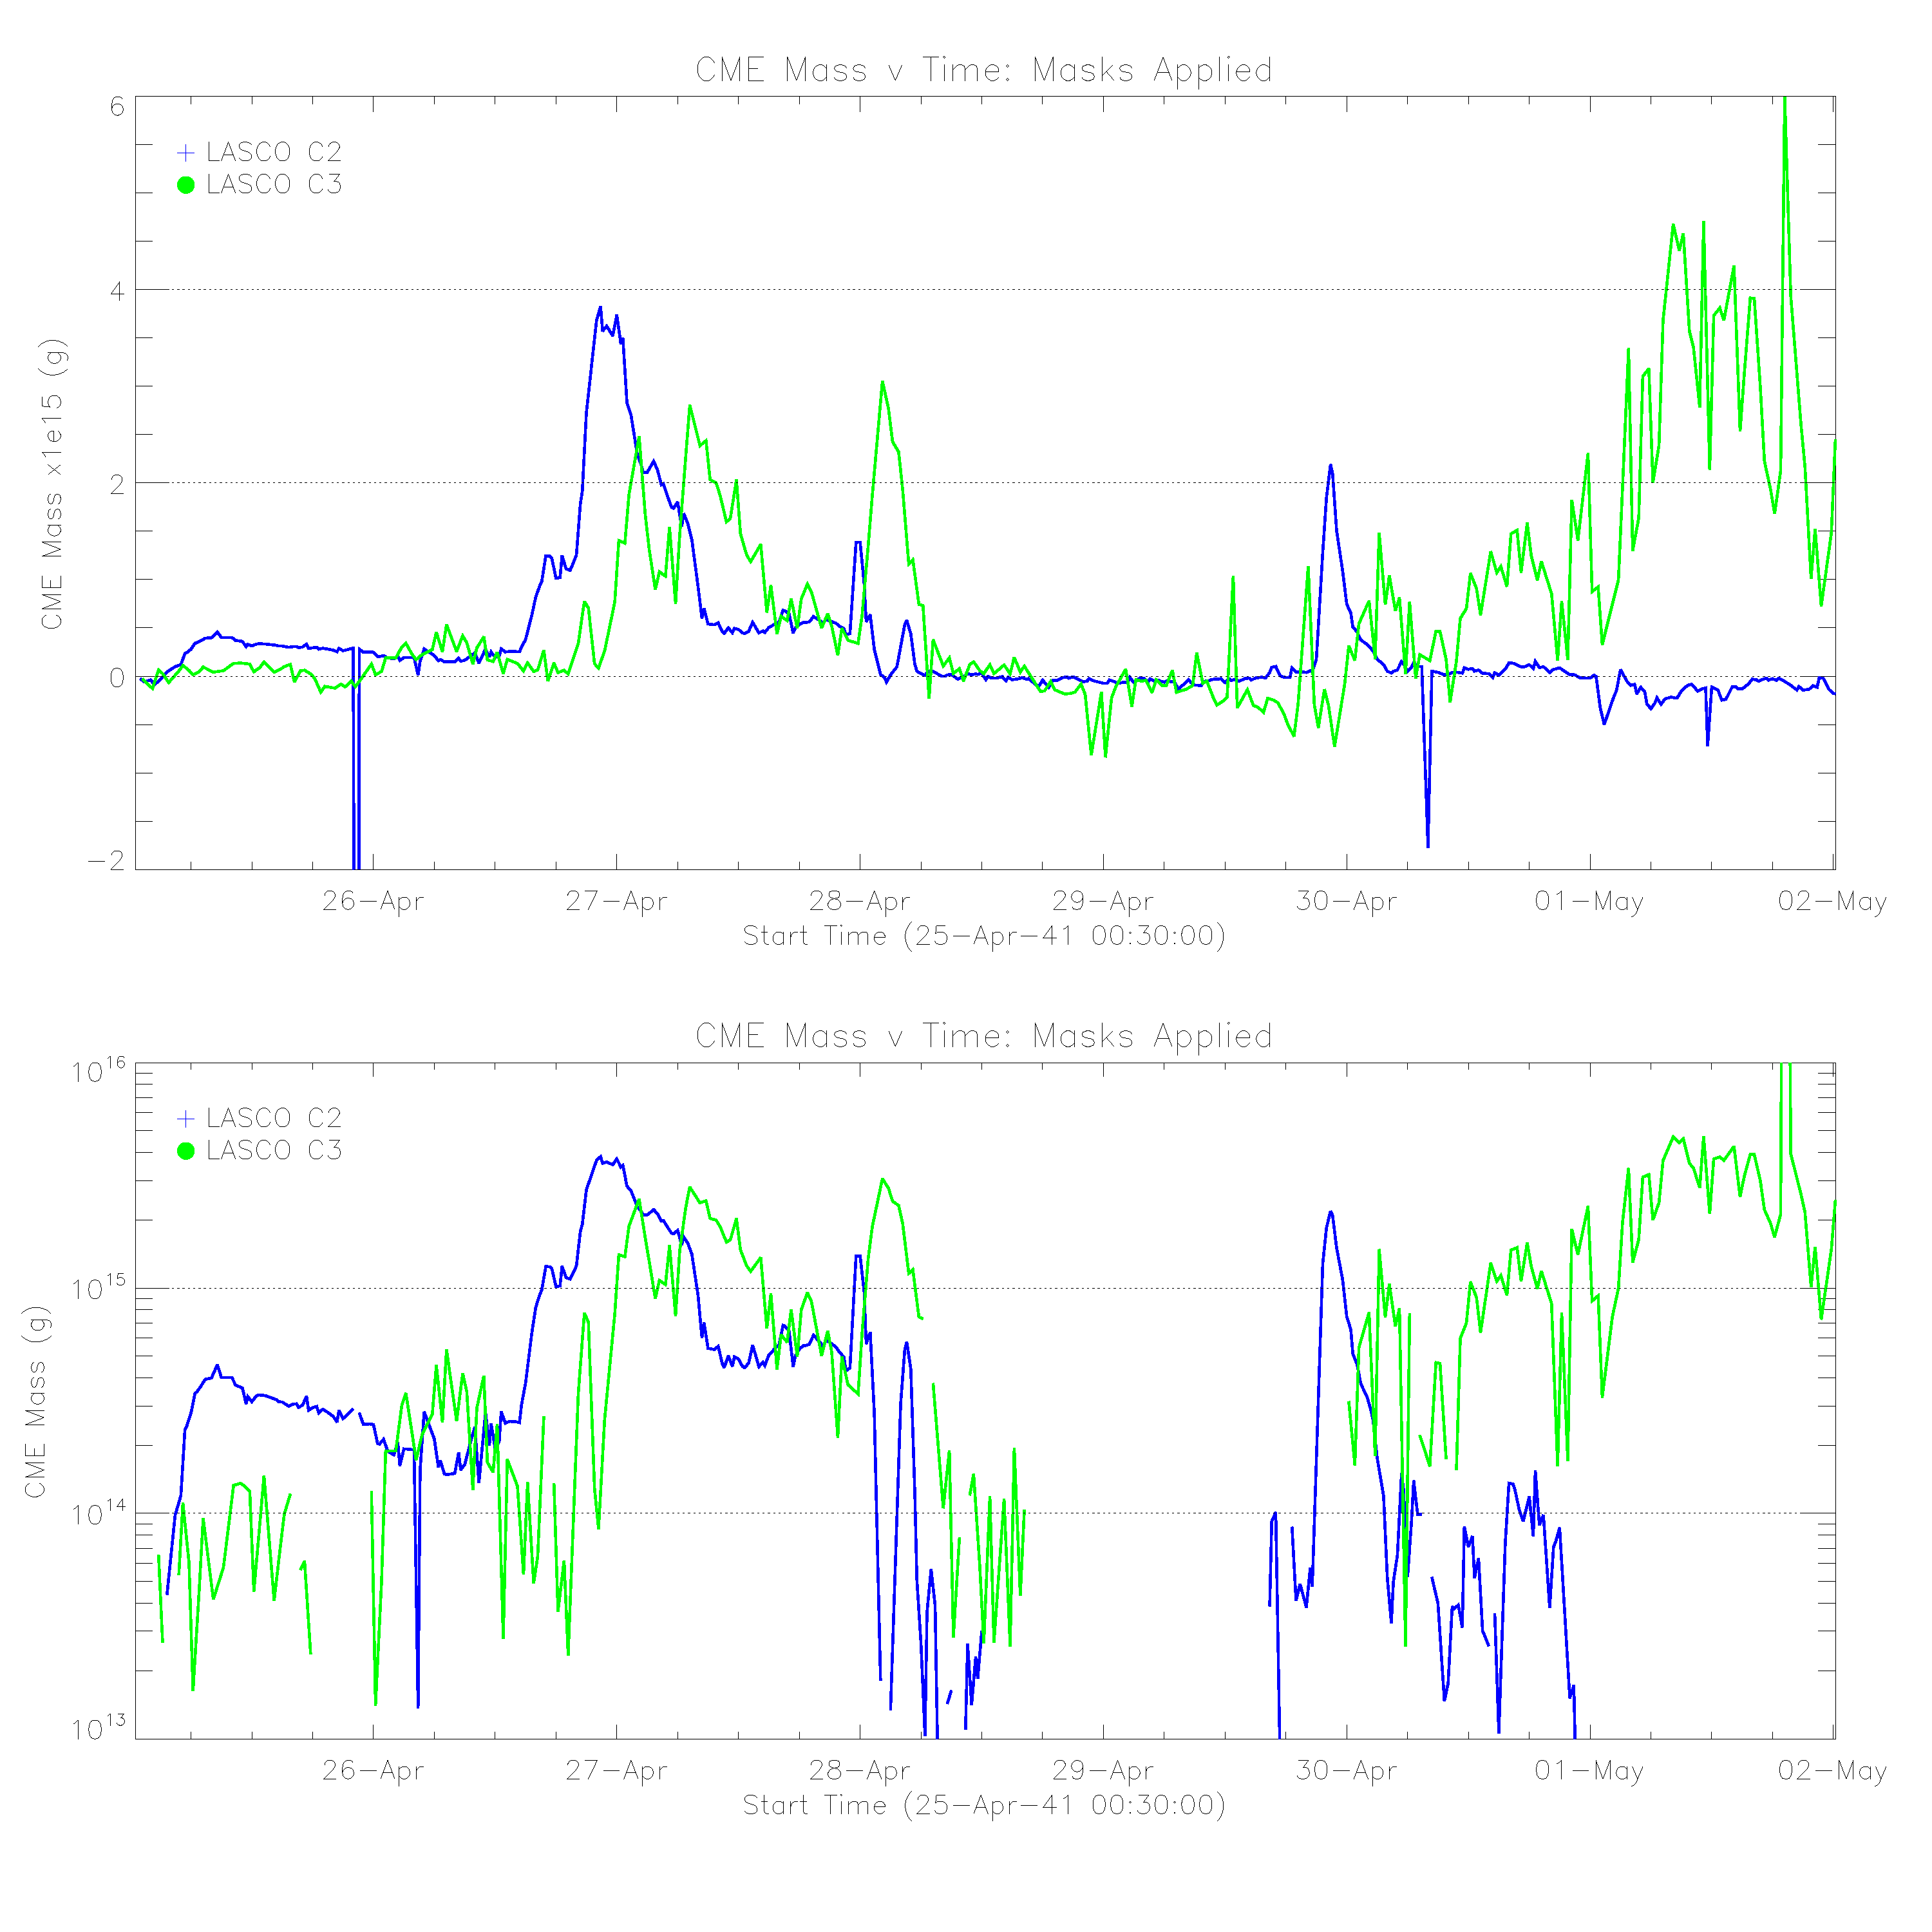
\includegraphics[scale=0.3, trim=7cm 2cm 7cm 4cm]{CME_MASSES_lin_log}
\caption[CME Mass automatic detection]{(Top) Mass estimates calculated using LASCO C2 and C3, and the detection masks of CORIMP. All images in the seven day observation sequence have been base-differenced, with the first image in the sequence used as a pre-event image. Representing mass on a linear scale shows clearly that the method results in reasonable estimates of CME mass. All CMEs are assumed to be propagating on the plane of sky (POS). 
(Bottom) Same data as Figure 1, with a logged y-axis. Logging the y-axis is more appropriate, given that CME masses tend to span approximately two orders of magnitude $10^{14}-10^{16}$\,g. However, with the logged axis, some issues with the method are highlighted e.g., the CME detection masks tend to capture spurious blobs (mass ejections, but not quite big enough to be regarded as CMEs). These blobs seem to occur in a lot of frames, making the background `quiet detections' level sit at $\sim$10$^{14}$\,g or higher. This is ok for larger CME masses however, the smaller CMEs with $M_{cme}\sim$10$^{14}$\,g will be swamped by this background detection. If we are to detect the whole range in mass, this background will have to come down. }
\label{fig:mass_v_time}
\end{center}
\end{figure}
%
%
%
%----------------------------------------------------%
%	 	Problem with background
%
There are a number of test which need to be performed in order to check that (i) the background subtraction is appropriate (ii) the mask has detected the right quantity of CME mass. At the moment the first image in the observation sequence is subtracted from all subsequent images. Not ideal, given that a CME eruption will change the background corona substantially. To avoid using the very first image, an algorithm needs to be employed to recognize a period of inactivity prior to eruption, and use an image (or an average of images) from this quiet period in the subsequent base difference.
%----------------------------------------------------%
%	 	 Test of the masking method
%
To check that (i) and (ii) are fulfilled we employ the fact that the following must be true
\begin{equation}
M_{mask} = M_{no\_mask} - M_{inverse\_mask}
\end{equation}
where $M_{mass}$ is mass calculated with the mask applied as normal, $M_{no\_mask}$ is just the total array summed, and $M_{inverse\_mask}$ is the CME masked with the remainder summed. The inverse mask is in Figure~\ref{fig:inverse_masks}. 
\begin{figure}[t!]
\begin{center}
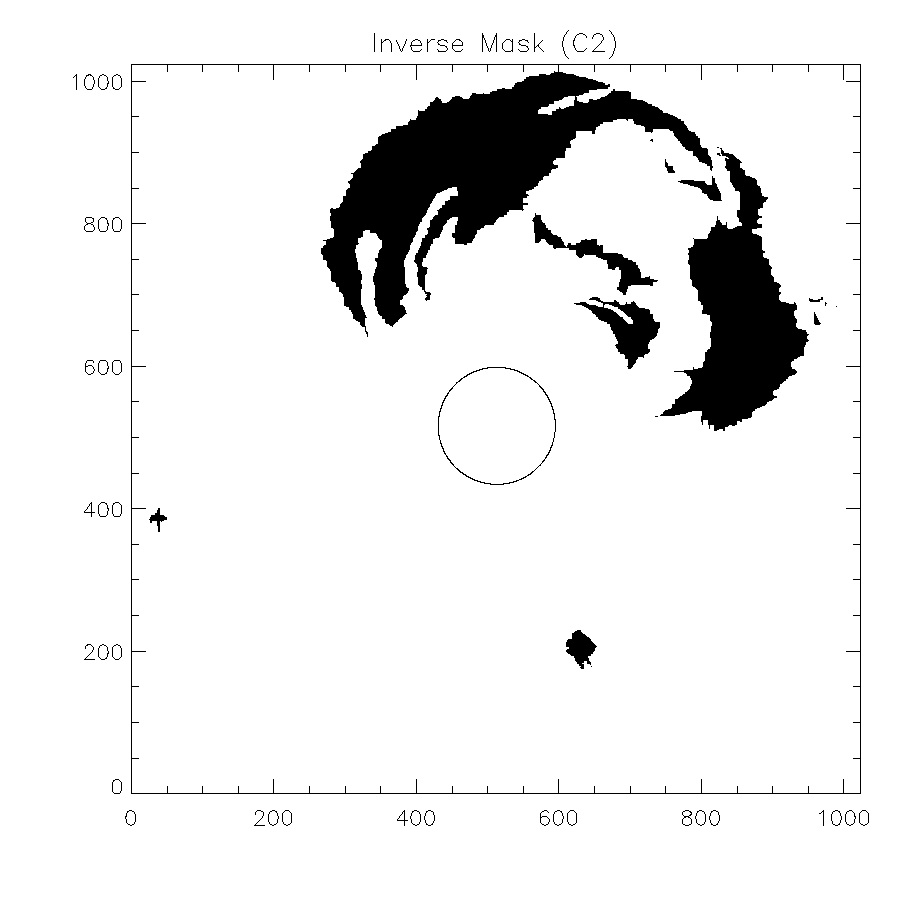
\includegraphics[scale=0.6, trim=0cm 2cm 0cm 0cm]{inverse_masks}
\caption{The inverse mask, allows everything \emph{but} the CME to be summed. Black circle is solar limb.}
\label{fig:inverse_masks}
\end{center}
\end{figure}

\begin{figure}[t!]
\begin{center}
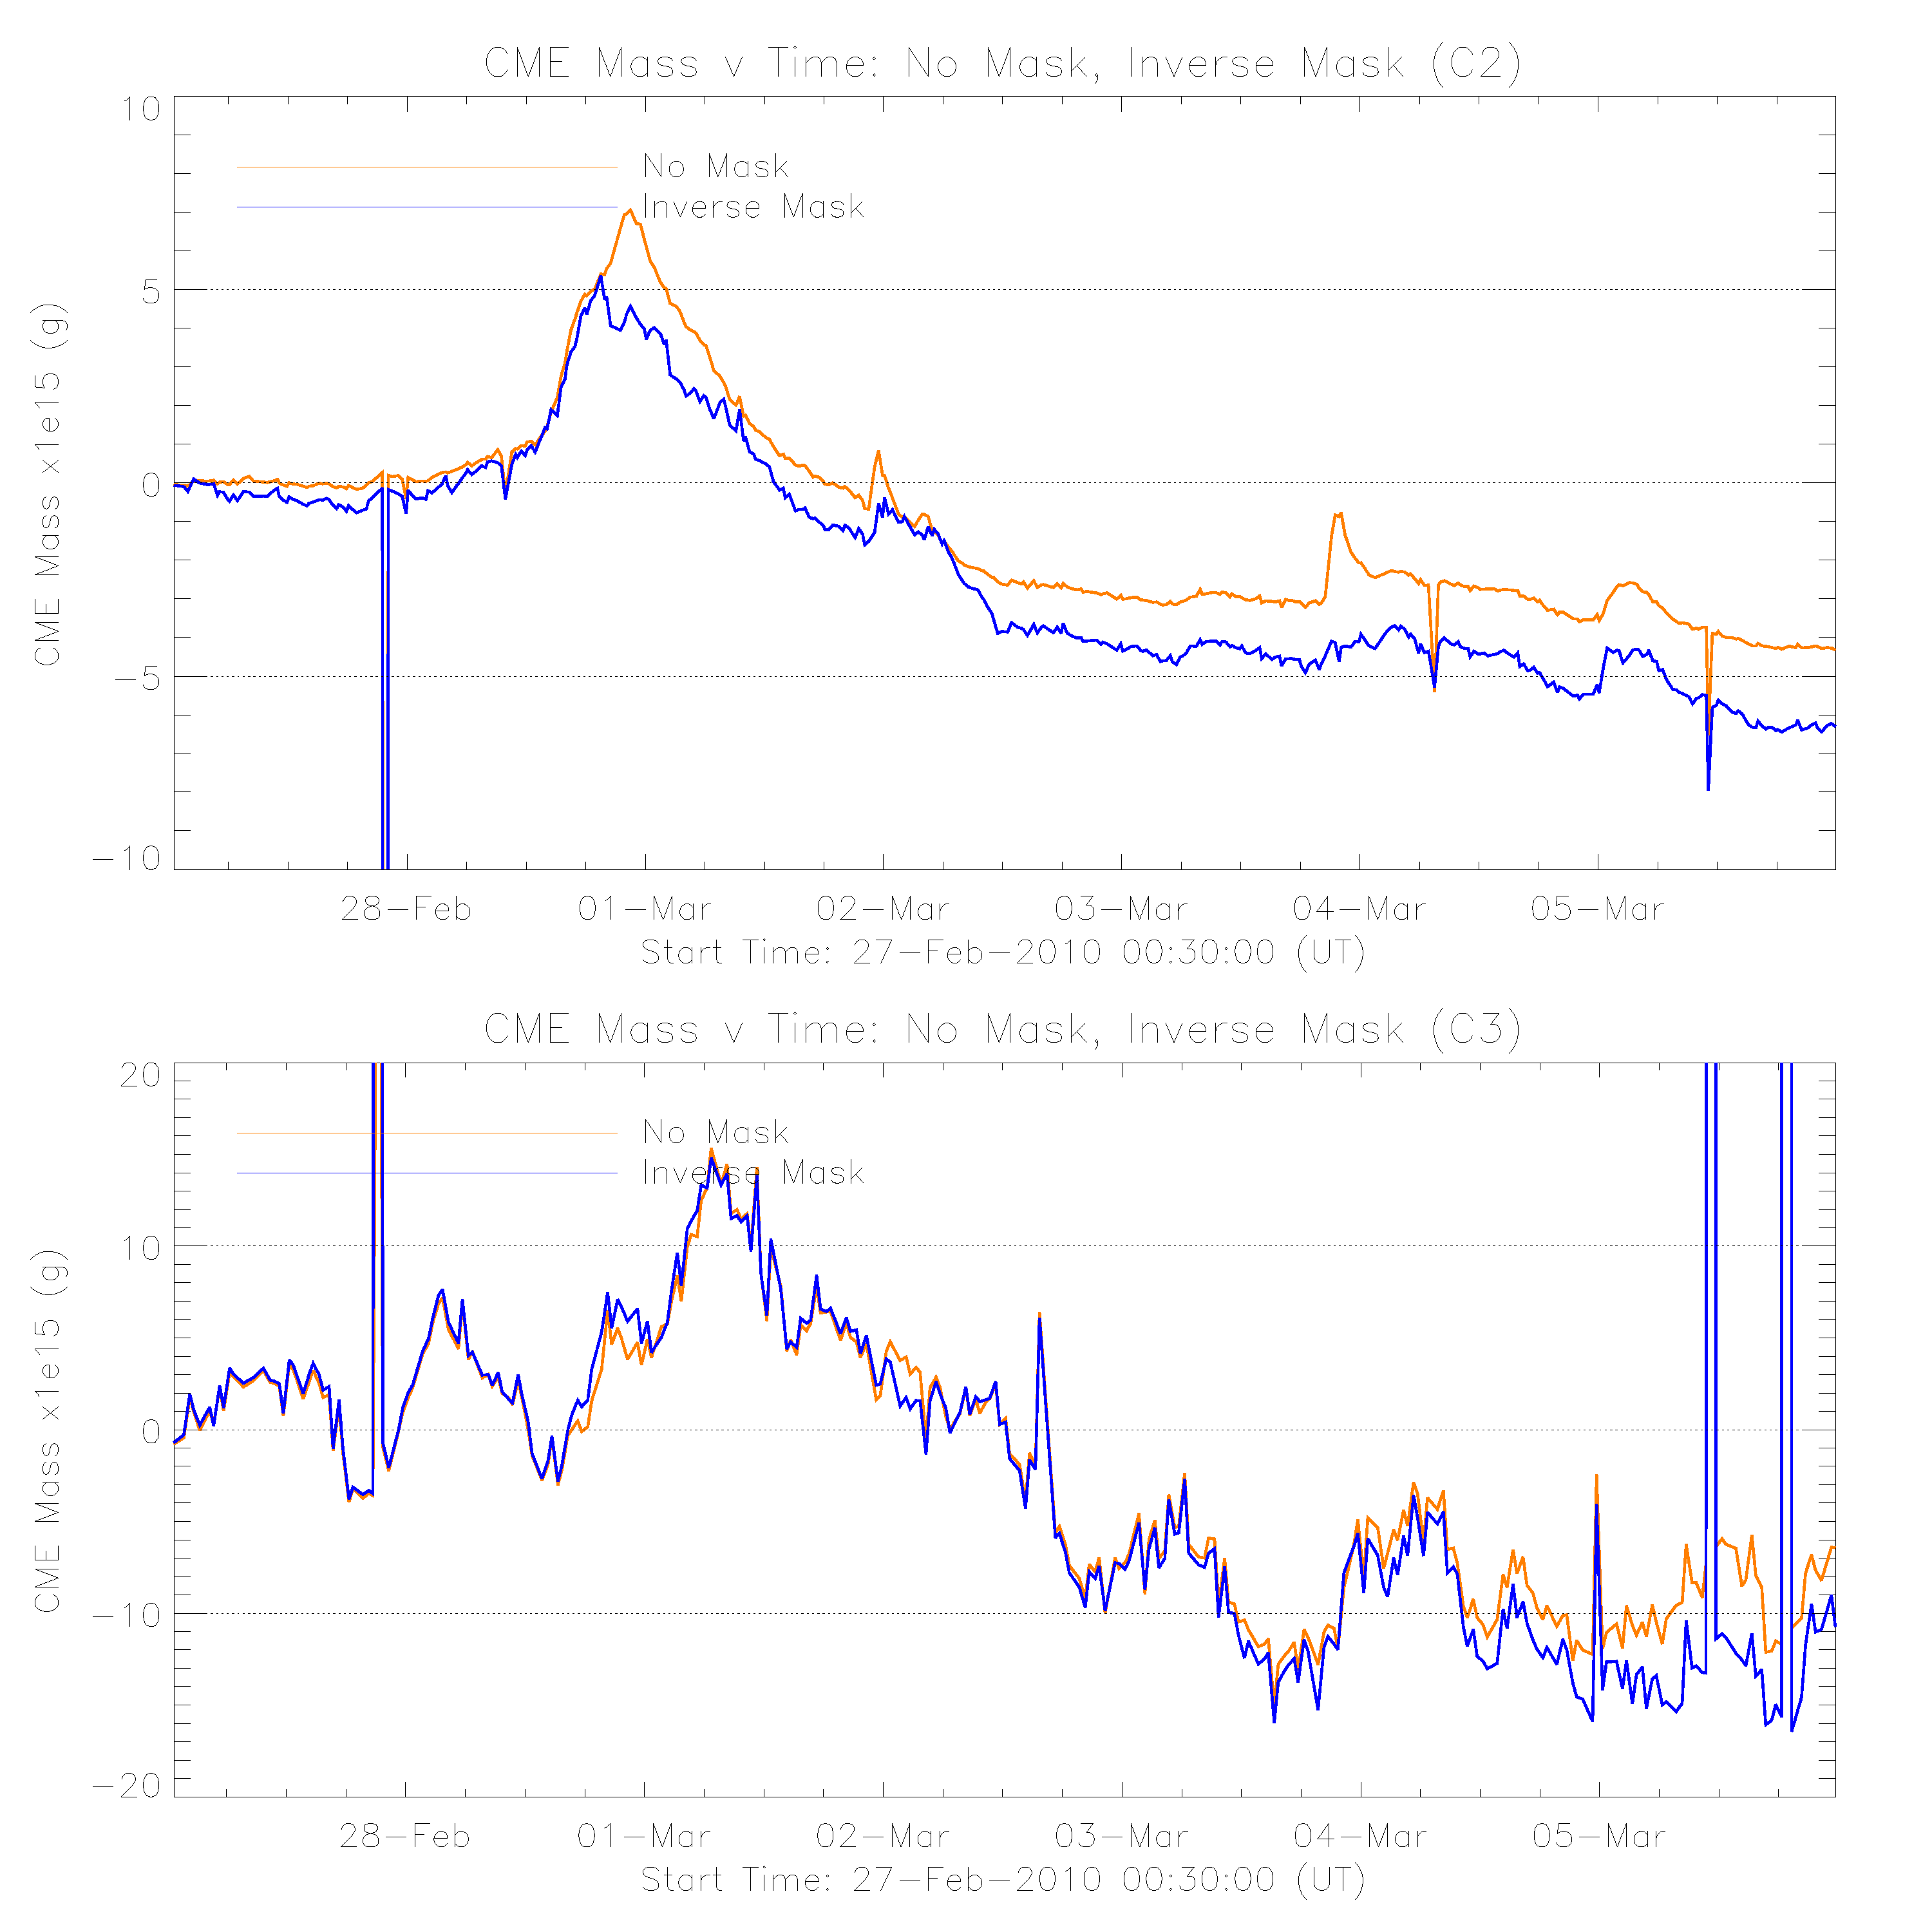
\includegraphics[scale=0.3, trim=0cm 2cm 0cm 1cm]{compare_masks_c2c3}
\caption{Time series of the mass obtained from using no mask and using the inverse mask. The data behave as expected, with the inverse mask being essentially the same as the no-mask but smaller by the CME mass. The drift towards negative values is symptomatic of a pre-event image (for base-difference) that is too bright. The discontinuous values are due to badly prepped images in the NRL archive.}
\label{fig:inverse_masks}
\end{center}
\end{figure}
We perform the time series again to calculate $M_{no\_mask}$ and $M_{inverse\_mask}$, shown in Figure~\ref{fig:inverse_masks}. They behave as expected, with the inverse-mask being essentially the same as the no-mask, but smaller by a roughly constant amount; this roughly constant amount should equal the CME mass. The effect of a single pre-event image used in the base-difference for the whole sequence is very apparent. In both C2 and C3 the masses grow toward increasingly negative values. This happens because the pre-event image is too bright and is a bad representation of the background corona over the observation sequences. In the intervening hours between start and end time a number of CMEs erupt. This will result in a dimming of the background corona over time as the corona becomes depleted or evacuated. This method has determined that condition (i) is not fulfilled, and is a good error check to see if an appropriate background has been chosen. To test condition (ii) we compare the difference of the blue and orange time series in Figure~\ref{fig:inverse_masks} with the time series calculated using the normal mask, the results are shown in Figure~\ref{fig:comparison}. The trends in both time series match, however they diverge as time increases. 
\begin{figure}[t!]
\begin{center}
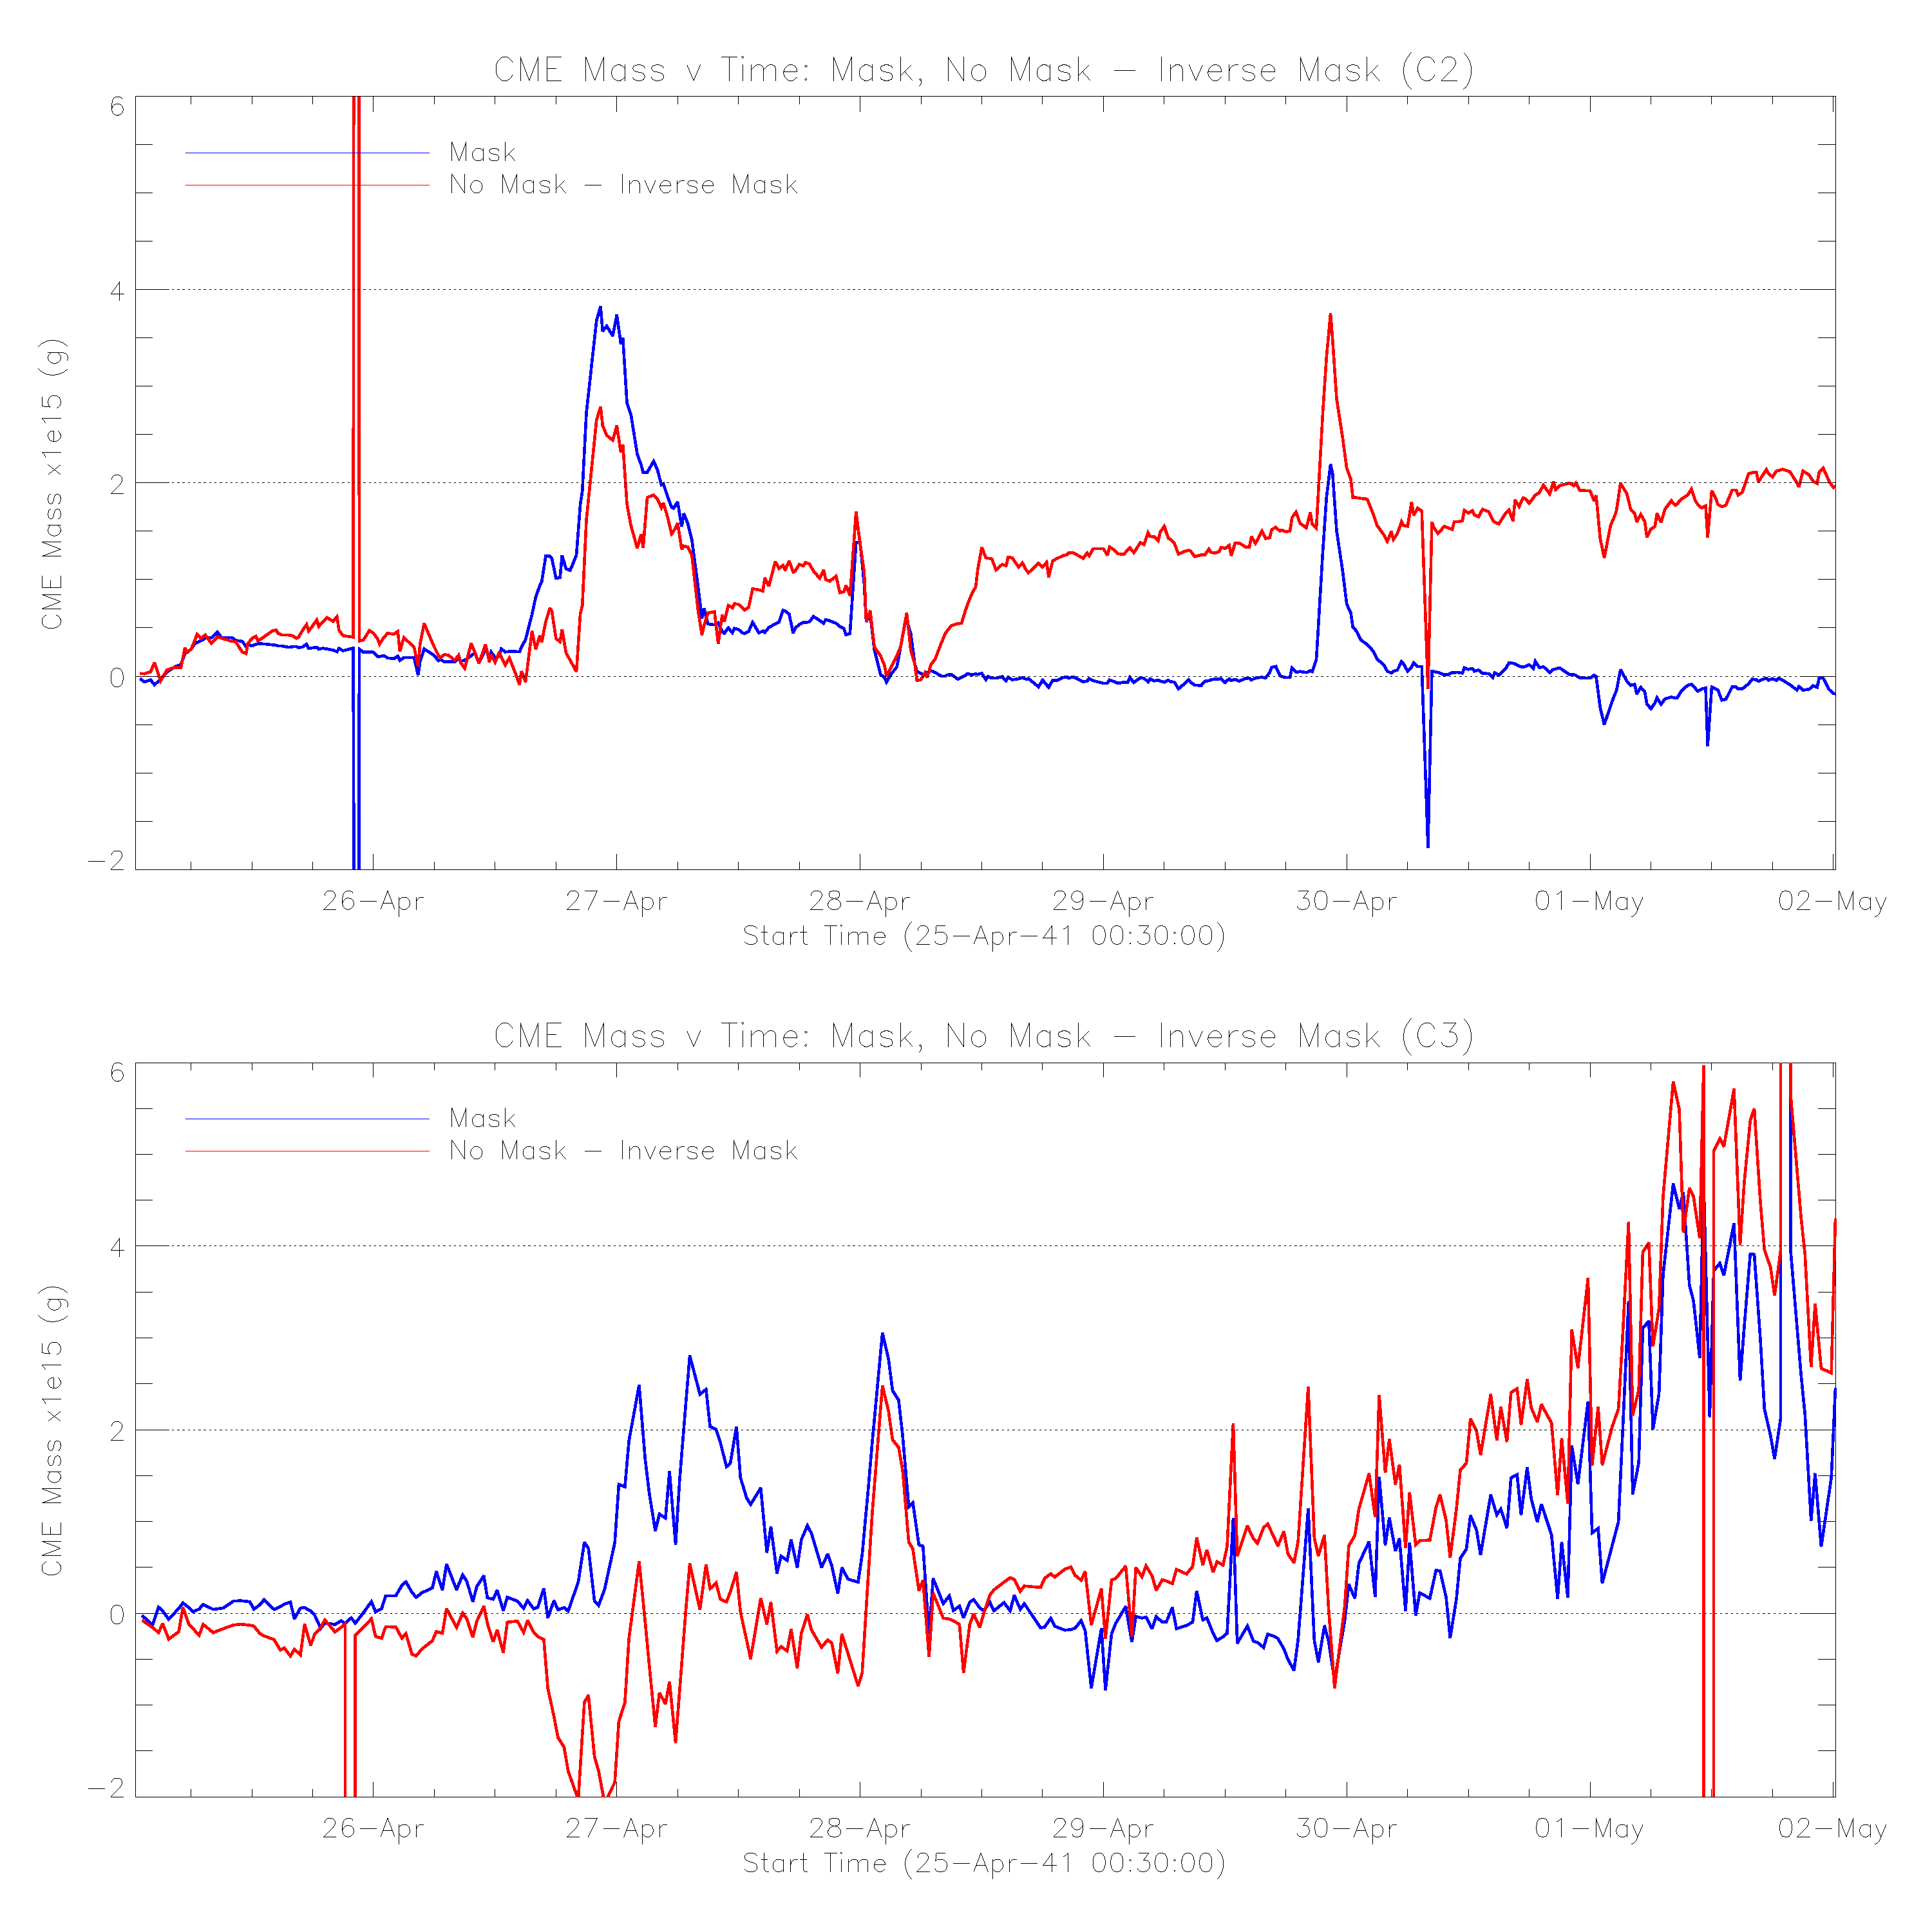
\includegraphics[scale=0.3]{mask_nomask_invmask_c2c3}
\caption{Comparison of the mass from masked images (blue) the no\_mask - inverse\_mask images (red) for C2 (upper) and C3 (lower). For both C2 and C3 the blue and red lines are a good match. The most obvious difference is the positive drift of the red line in C2, due to an excess background brightness subtracted in the base-differencing.}
\label{fig:comparison}
\end{center}
\end{figure}
The over-bright pre-event image used in the base difference is drawing the background values in no-mask and invert-mask into negative values. The blue line in Figure~\ref{fig:inverse_masks} (upper panel) should sit at zero, while the orange line should only show positive values when a CME is in the frame. The fact that they both drift into the negative means they will result in a positive excess when subtracting the two.
Algebraically, the procedure resulting in the red line in Figure~\ref{fig:comparison} is as follows:
\begin{equation}
y = (img - pre) - (img - pre)\times mask_{inverse}
\end{equation}
where $img$ is the current image and $pre$ is pre-event image; $img - pre$ represents a base difference. $mask_{inverse}$ is the inverted mask e.g., Figure~\ref{fig:inverse_masks}. Ideally, equation (2) would result in
\begin{equation}
y = M_{cme} - 0
\end{equation}
However due to excess brightness in the pre-event image we end up with a negative mass value $M_{neg}$ combined with the cme mass $M_{cme}$
\begin{equation}
y = (M_{neg} + M_{cme})  - M_{neg}
\end{equation}
Since $M_{neg} < (M_{neg} + M_{cme}   ) < 0$, we end up with $y$ value that is positive and larger than $M_{cme}$. Of course, if the pre-event image were chosen appropriately we would just have equation (3), no problem. It's interesting to note that the difference between the blue and red line in Figure~\ref{fig:comparison} is a measure of how much the background corona changed over time; it also a measure of how well chosen the background image is for the base-difference. If the lines diverge consistently, too much background brightness has been extracted from the images. The effect is not as pronounced in C3 for the observation sequence, probably because the CME does not perturb the background corona at this height range as much as it does at lower heights (in C2 FOV). Hence the analysis resulting in Figure~\ref{fig:comparison} are a way of confirming that criteria (i) and (ii) are fulfilled.

There are a number of questions and issues that need to be addressed if the automatic mass detection is to produce reliable results:
\begin{itemize}
\item Removal of the spurious blobs in the quiet-time masks. Background values need to be brought to a maximum of $10^{13}$\,g, this will ensure detection of even small CMEs with masses of $\sim$$10^{14}$\,g. A criteria for the removal of these blobs could be to ignore detections smaller than a threshold angular width i.e., set to zero all features with angular width $<40^{\circ}$
\item An algorithm to choose an appropriate prevent image needs to be implemented. An average of a set of quiet images before CME detection is a possibility. In this case the algorithm will need to identify a CME start time and then to check for the presence of quiet images before this start time. 
\item What mass value should be taken as being representative of the CME mass? Is it appropriate to take the maximum mass value detected during the time interval when the CME is present? If so, should the maximum mass be taken from C2 or C3?
\end{itemize}
The last item here will require a a number of tests to be performed on which telescope can provide the most reliable mass estimate. Primarily, C3 would seem like the most appropriate, since the large field-of-view (FOV) can contain all CME material i.e., there will be none hidden by the occulter, as can happen in the C2 FOV. However, C3 is more susceptible to plane-of-sky (POS) errors e.g., if CME is not actually on POS, the uncertainties introduced by assuming it \emph{is} on POS are worse for C3. There main pros and cons of each coronagraph are
\begin{itemize}
\item C2 \hfill \\
-Pro: CME is closer to POS \\
-Con: Mass is hidden behind disk
\item C3 \hfill \\
-Pro: FOV is large enough to view all CME (smaller mass-hiding)\\ 
-Con: Very bad POS effects
\end{itemize}
These may be addressed by a study of the Thomson scattering geometry of the light received by each telescope.

Finally, the inherent uncertainties on the CME mass a the most serious threat to the feasibility of automatic mass detection. Realistically, we can only give an order of magnitude estimate e.g., CME mass is somewhere between $10^{14}-10^{15}$\,g or $10^{15}-10^{16}$\,g etc. One idea is a CME mass classification into ranges such as
\begin{itemize}
\item A Mass: $10^{13}-10^{14}$\,g
\item B Mass: $10^{14}-10^{15}$\,g
\item C Mass: $10^{15}-10^{16}$\,g
\item C+ Mass: $>10^{16}$\,g (on the off chance that mass is slightly above C)
\end{itemize}
With such a system you could say there was a \textquoteleft C' mass CME on such a date and time, without having to quote some uncertain mass estimate. The uncertainties might result in the mass transcending two classes, in that case you could then quote \textquoteleft BC' mass. In practice, such large ranges may be the only way in which CME mass values can be presented in a catalogue. Despite such limitations, this may be useful to any user wishing to search for events that have small, intermediate, or large energies.

\subsubsection{EUV Dimming Mass with AIA}

Read Aschwanden study, compare it to AIA.

This study has never been performed with the superior time and space resolution of AIA. Furthermore, the larger number of passbands with AIA can provide more reliable DEM estimates. Such an analysis may reveal correlations between CME mass evacuation and flare rise time (private commination, Angelos Vorulidas).


\section{Coronal Shocks and Radio Bursts}

\subsection{Principle results}
The second goal of this thesis was to increase the understanding of CME-driven shocks and show the relationship amongst the various shock observables. A combination of white-light, EUV, and radio imaging showed CBFs and radio bursts have a common origin in a shock, and that this shock was driven by the CME flank. In this chapter, I will summarise and conclude this research and outline the future of this study

\subsection{Future Work}

\subsubsection{Herringbone Statistics and the Hough Transform}

\subsubsection{100 CME Challenge}


